% !TEX root = ../review.tex
\begin{frame}
\frametitle{MAligner\nocite{maligner}: Общие сведения}
Два подхода:
\begin{enumerate}
  \item На основе алгоритма Смита-Ватермана
  \begin{itemize}
    \item Построение множества выравниваний на референсе
    \item Определение значимых выравниваний - M-Score
  \end{itemize}
  \item На основе индексации
\end{enumerate}
\end{frame}

\begin{frame}
\frametitle{MAligner: Алгоритм динамического программирования}

Пусть имеются два выравненных участка c n и m пропущенными фрагментами длины r и m на референсе и карте соотвественно.
Тогда выравнивание имеет следующее значение:

\begin{gather*}
Score(q, r, m, n) = S(q, r) + C_q \,m + C_r \, n \\
S(q, r) = \bigg(\frac{q - r}{\sigma(r)}\bigg)^2 \\
\sigma(r) = \max(\alpha \, r, \sigma_{min})
\end{gather*}
$C_q$ - штраф за пропущенные фрагменты на карте \\
$C_r$ - штраф за пропущенные фрагменты на референсе \\
$\sigma_{min}$ - для фрагментов малой длины, ошибка больше \\
$\alpha$ - доля референса, которая будет использовать как стандартное отклонение
\end{frame}

\begin{frame}
\frametitle{MAligner: M-Score - значимость выравнивания}

Предложена оценка M-Score для определения значимости выравнивания:

\begin{gather*}
  m_{\mathcal{A}} = \underset{A \in \mathcal{A}}{median}\{Score(A)\} \\
  MAD_{\mathcal{A}} = \underset{A \in \mathcal{A}}{median}\{ | Score(A) - m_{\mathcal{A}}|\} \\
  M-Score_{\mathcal{A}}(A) = \frac{Score(A) - m_{\mathcal{A}}}{MAD_{\mathcal{A}}}
\end{gather*}

$Score(A)$ - значение выравнивания $A$

$\mathcal{A}$ - 100 лучших выравниваний по Score(A)
\end{frame}


\begin{frame}
\frametitle{MAligner: Алгоритм на основе индексов}
Работает в предположении, что в карте не могут быть пропущенные разрезы:
\begin{enumerate}
  \item Выбирается k и строятся всевозможные k-tuple на референсе длины меньше k - $\mathcal{K}$ и сортируем его по длине.
  \item Далее строится по множеству $\mathcal{K}$ граф, где вершины - k-tuple, а рёбрами соединяем те k-tuple, у которых граничные разрезы совпадают.
  \item У входной карты берём k-tuple и бинарным поиском по длине в $\mathcal{K}$ ищем схожие k-tuple.
  \item Для каждого найденного k-tuple  запускаем поиск в ширину по графу, при чём идём только по тем вершинам, длины которых $C$ удовлетворяют очередному фрагменту карты длины $c_q$:
  \begin{gather*}
     c_q - max(\alpha \, c_q, \beta) \le C \le c_q + max(\alpha \, c_q, \beta)
  \end{gather*}
  \item Получаем набор выравниваний.
\end{enumerate}
\end{frame}

\begin{frame}
\frametitle{MAligner: Результаты}
  Данные без ошибок:
  \begin{figure}
    \centering
    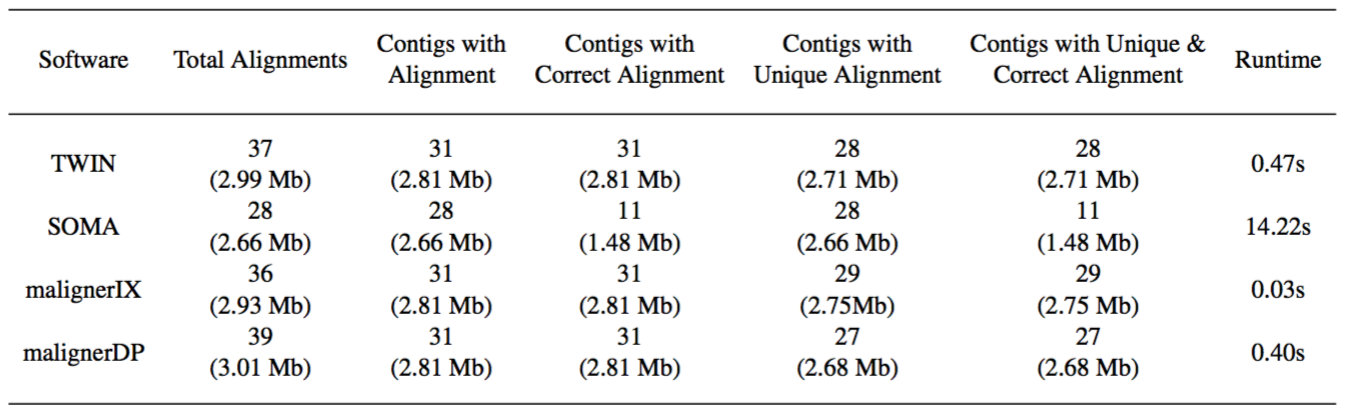
\includegraphics[width = 0.9\textwidth]{maligner/without_errors}
  \end{figure}
  Данные с ошибками:
  \begin{figure}
    \centering
    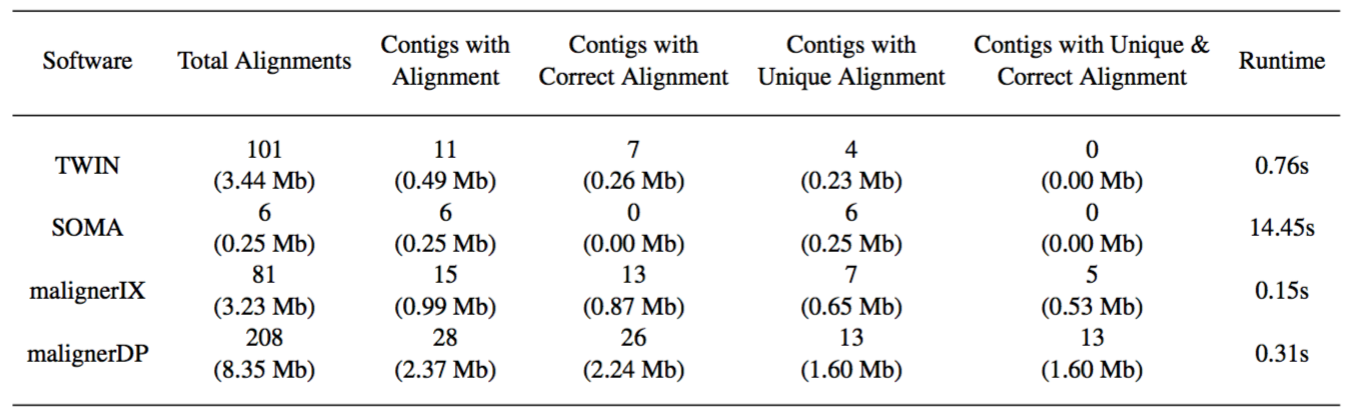
\includegraphics[width = 0.9\textwidth]{maligner/with_errors}
  \end{figure}

\end{frame}
